%%=========================================
\chapter{Results}\label{AppendixA}
This appendix displays all results that were not relevant enough to be a part of the results chapter.

\section{Experiment 2}
\begin{figure}[htbp]
    \centering
    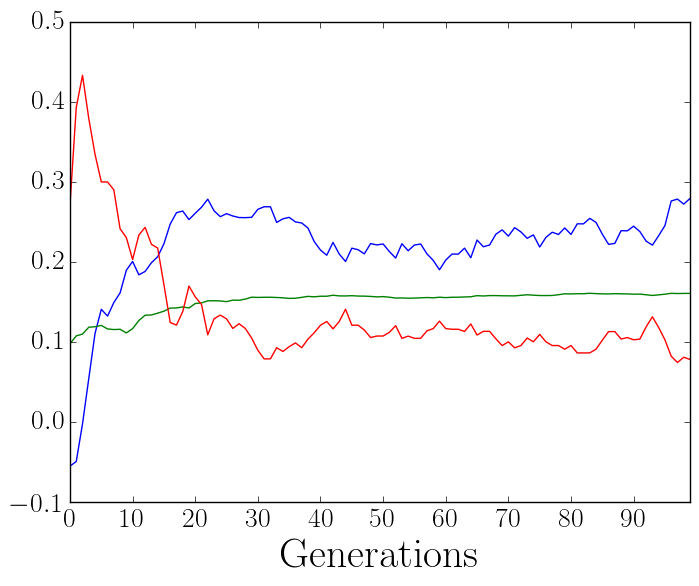
\includegraphics[width=0.49\linewidth]{fig/Results/Exp2/Genes1}
    \caption{Genes from experiment 2. Green: Average probability of conducting parent-child dialogues. Blue: Average learning rate. Red: Average probability of acting extrovertly.}
    \label{fig:Genes2}
\end{figure}

\clearpage
\section{Experiment 3}
\begin{figure}[htbp]
    \centering
    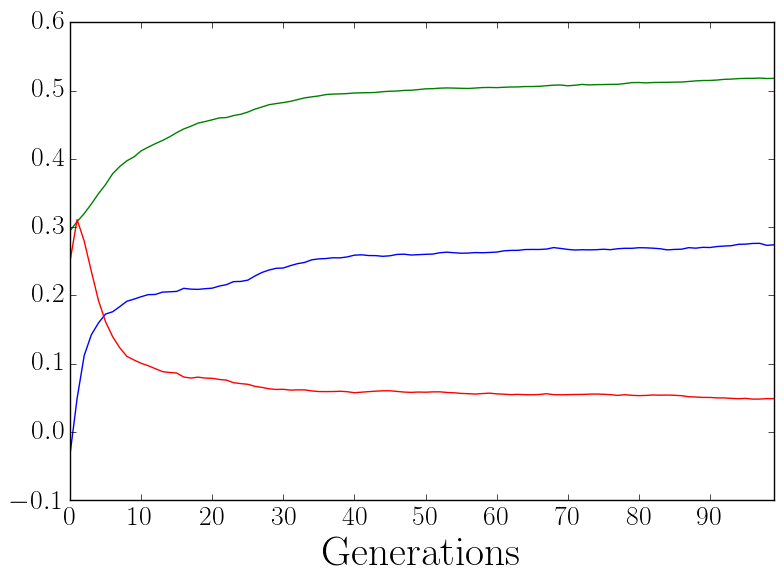
\includegraphics[width=0.49\linewidth]{fig/Results/Exp3/Genes1}
    \caption{Genes from experiment 3. Green: Average probability of conducting parent-child dialogues. Blue: Average learning rate. Red: Average probability of acting extrovertly.}
    \label{fig:Genes3}
\end{figure}


\section{Experiment 4}

\begin{figure}[htbp]
    \centering
    \subfigure[Green: Average vocabulary size. Blue: Successful dialogues divided by total number of dialogues.]{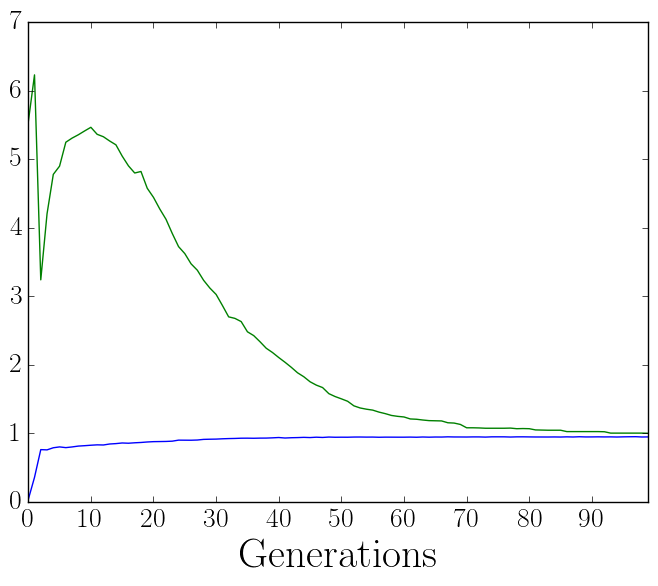
\includegraphics[width=0.49\linewidth]{fig/Results/Exp4/Vocabulary1}}
    \hfill
    \subfigure[Green: Average probability of conducting parent-child dialogues. Blue: Average learning rate. Red: Average probability of acting extrovertly.]{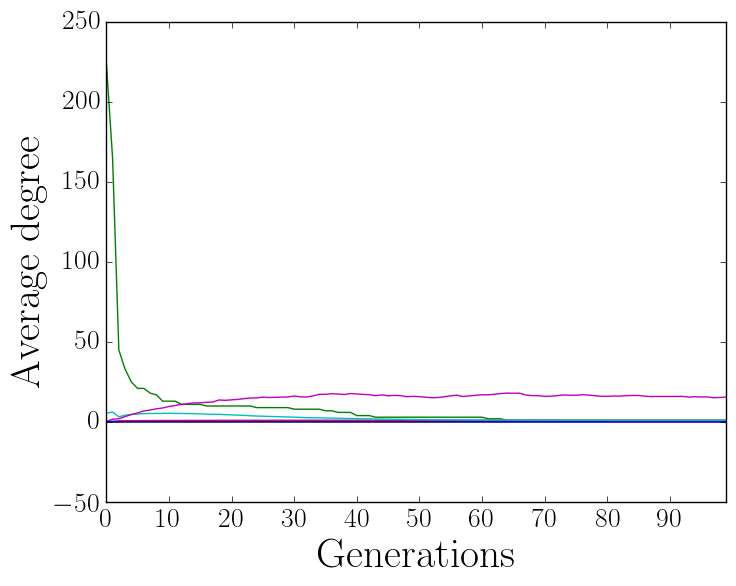
\includegraphics[width=0.49\linewidth]{fig/Results/Exp4/genes1}}
    \caption{Results from experiment 4.}
\end{figure}
\begin{figure}
    \subfigure[The social network at generation 5.]{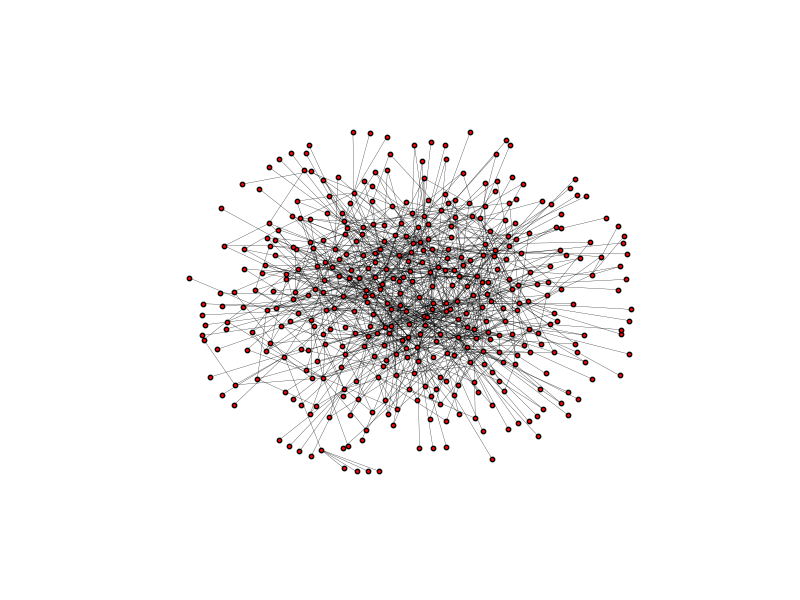
\includegraphics[width=0.49\linewidth]{fig/Results/Exp4/_graph5}}
    \hfill
    \subfigure[The social network at generation 20.]{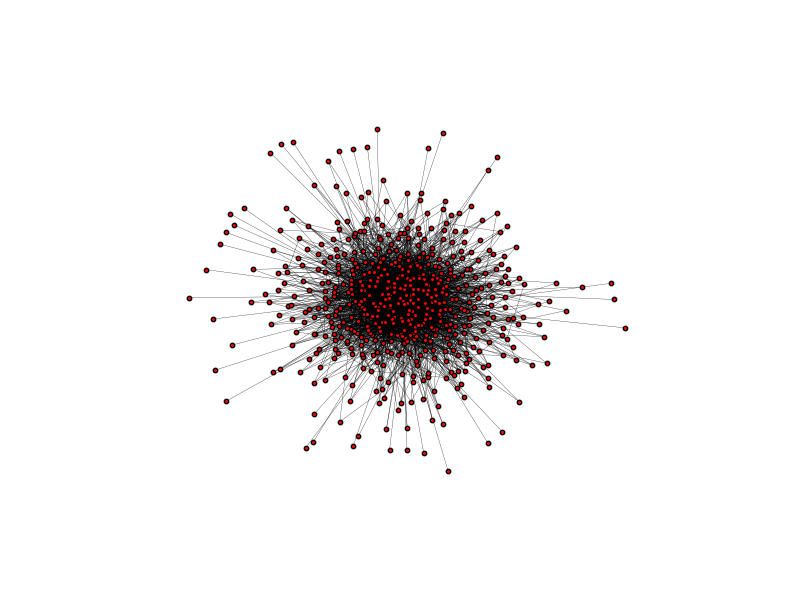
\includegraphics[width=0.49\linewidth]{fig/Results/Exp4/_graph20}}
    \par \bigskip
    \subfigure[The social network at generation 40.]{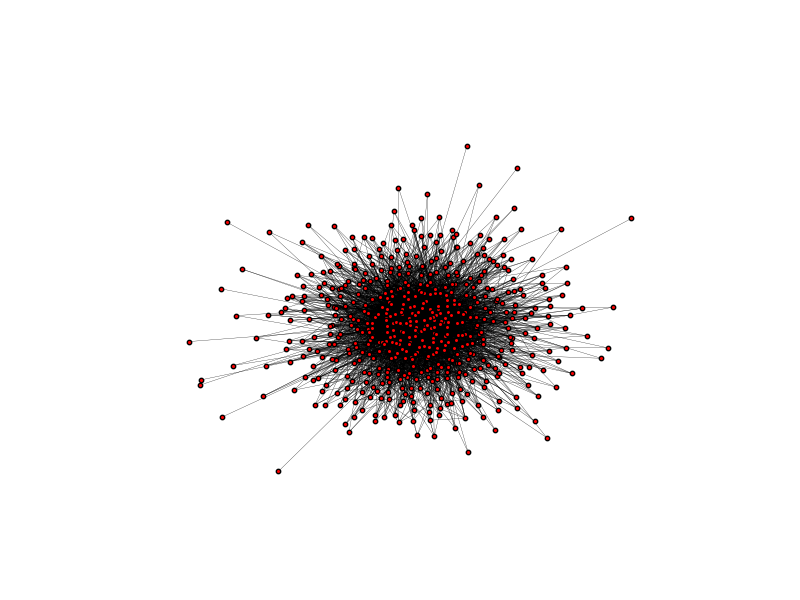
\includegraphics[width=0.49\linewidth]{fig/Results/Exp4/_graph40}}
    \hfill
    \subfigure[The social network at generation 100.]{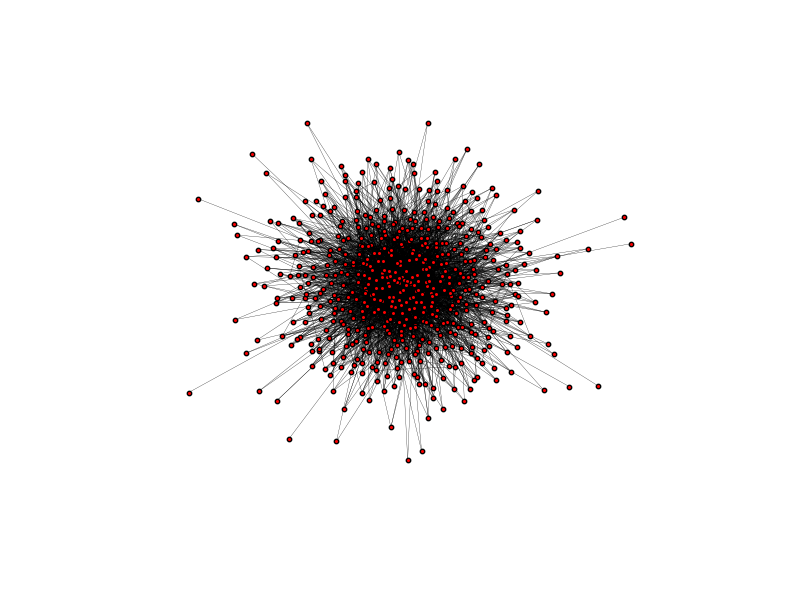
\includegraphics[width=0.49\linewidth]{fig/Results/Exp4/_graph100}}
    \caption{Results from experiment 4.}
    \label{fig:Appendix4}
\end{figure}

\section{Experiment 5}

\begin{figure}[htbp]
    \centering
    \subfigure[Social network at generation 20]{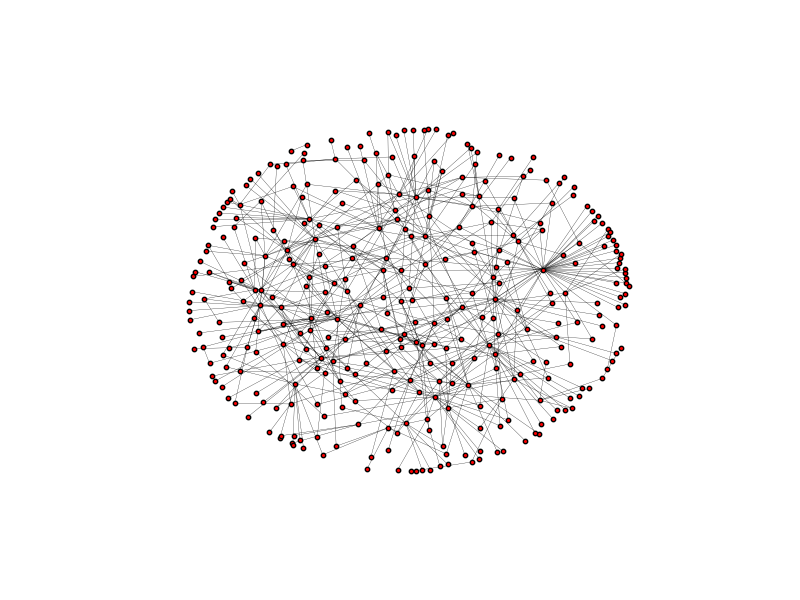
\includegraphics[width=0.49\linewidth]{fig/Results/Exp5/_graph20}}
    \hfill
    \subfigure[Social network at generation 150]{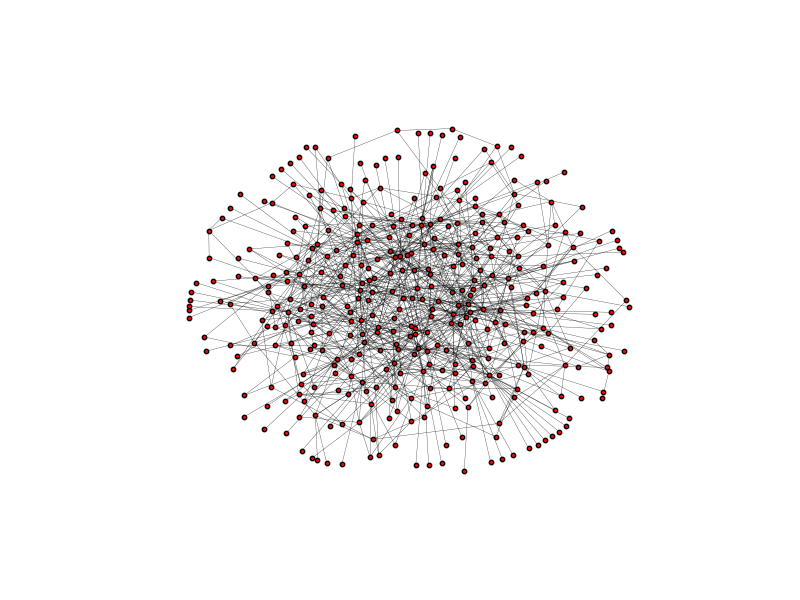
\includegraphics[width=0.49\linewidth]{fig/Results/Exp5/_graph150}}
    \par \bigskip
    \subfigure[Green: Average probability of conducting parent-child dialogues. Blue: Average learning rate. Red: Average probability of acting extrovertly.]{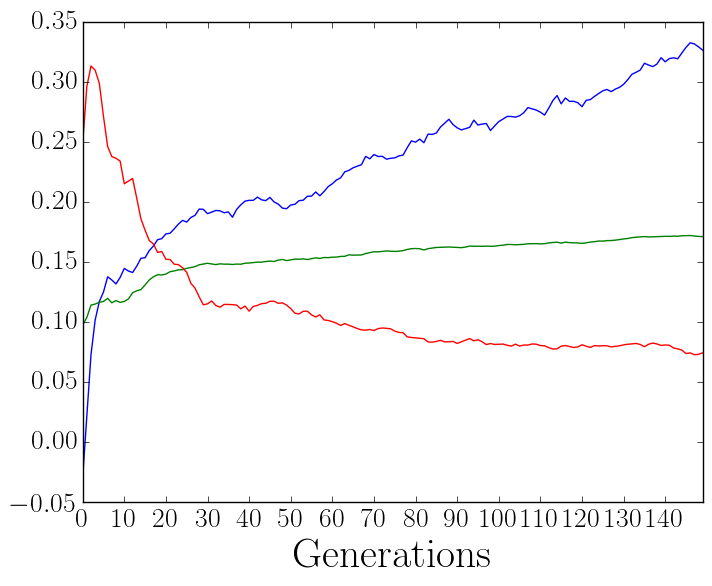
\includegraphics[width=0.5\linewidth]{fig/Results/Exp5/Genes1}}
    \caption{Results from experiment 5}
\end{figure}

\clearpage
\section{Experiment 6}

\begin{figure}[htbp]
    \centering
    \subfigure[Green: Average probability of conducting parent-child dialogues. Blue: Average learning rate. Red: Average probability of acting extrovertly.]{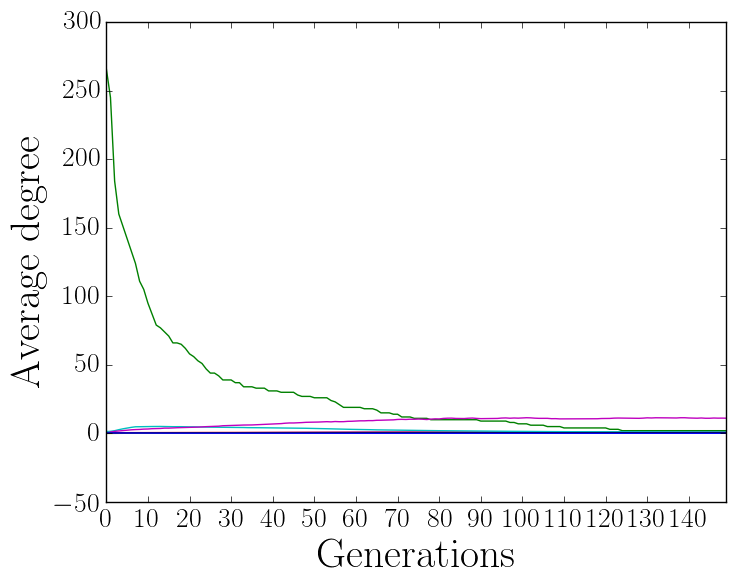
\includegraphics[width=0.5\linewidth]{fig/Results/Exp6/Genes1}}
    \hfill
    \subfigure[The social network at generation 5.]{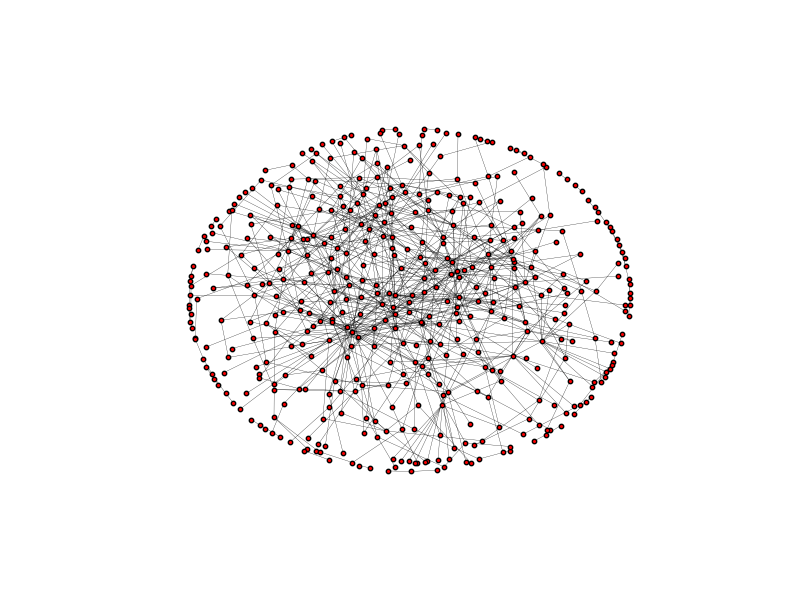
\includegraphics[width=0.49\linewidth]{fig/Results/Exp6/_graph5}}
    \par \bigskip
    \subfigure[The social network at generation 20.]{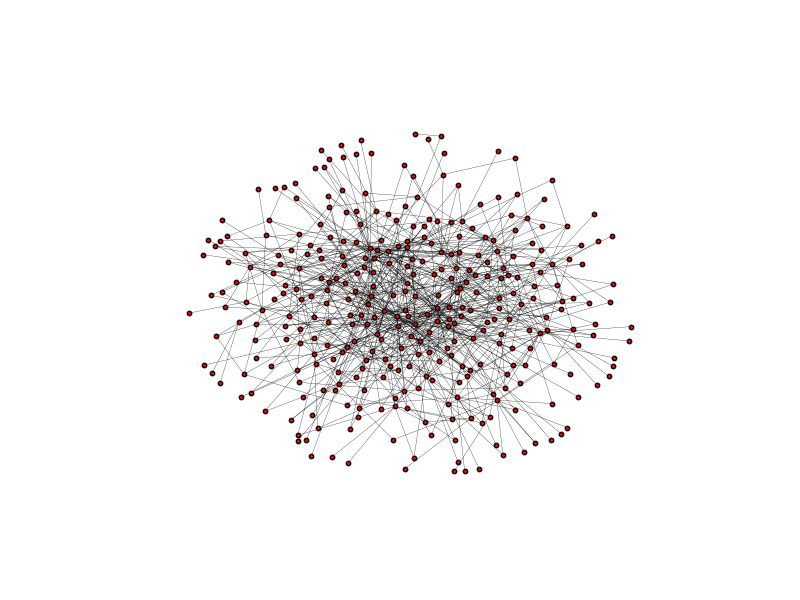
\includegraphics[width=0.49\linewidth]{fig/Results/Exp6/_graph20}}
    \hfill
    \subfigure[The social network at generation 100.]{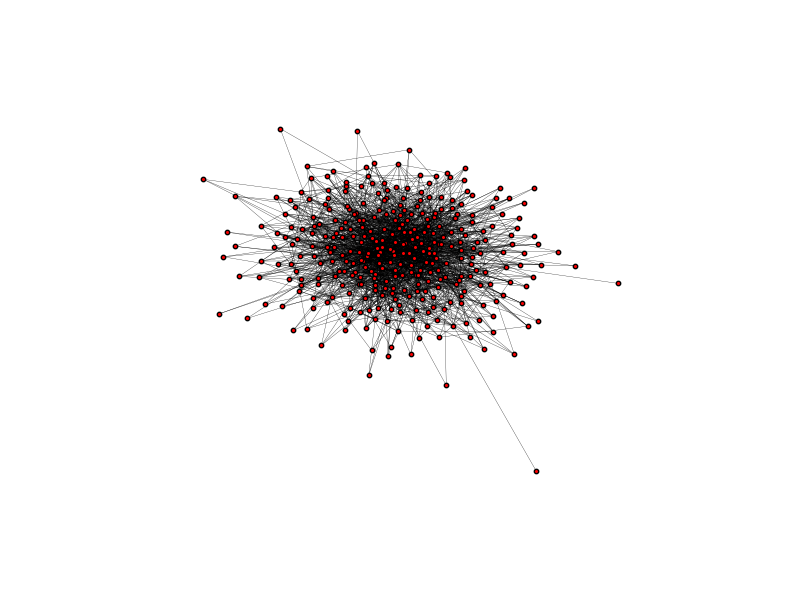
\includegraphics[width=0.49\linewidth]{fig/Results/Exp6/_graph100}}
    \caption{Results from experiment 6 with $k = 0.95$ and $n = 0.7$.}
\end{figure}

\clearpage
\begin{figure}[htbp]
    \centering
    \subfigure[The average fitness.]{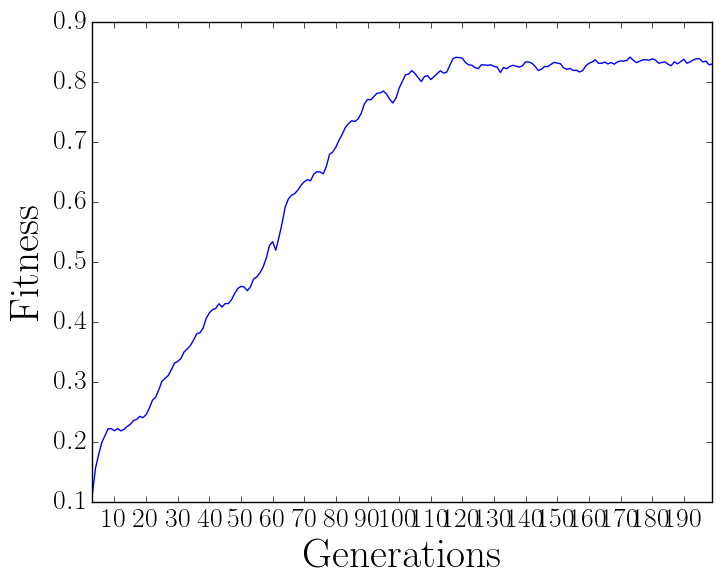
\includegraphics[width=0.49\linewidth]{fig/Results/Exp6.1/Fitness1}}
    \hfill
    \subfigure[The average degree.]{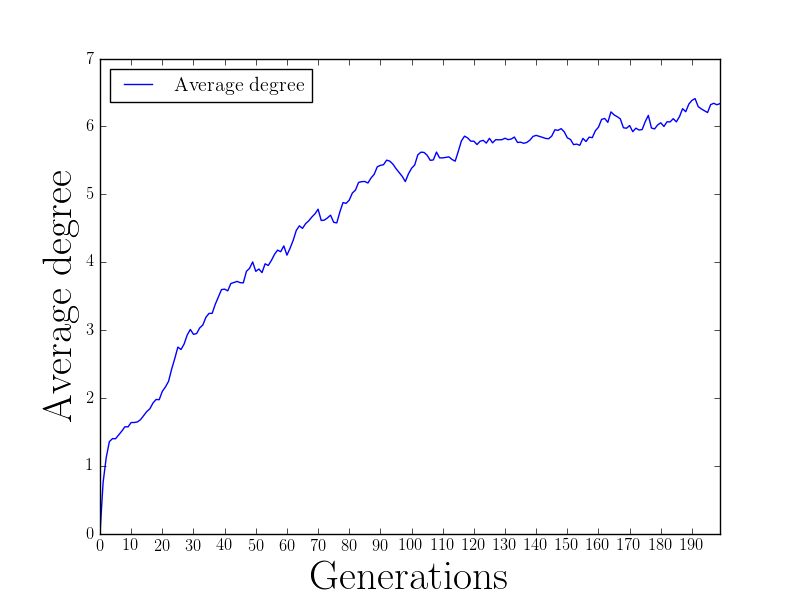
\includegraphics[width=0.49\linewidth]{fig/Results/Exp6.1/Degree1}}
    \par \bigskip
    \subfigure[Green: Average vocabulary size. Blue: Successful dialogues divided by total number of dialogues.]{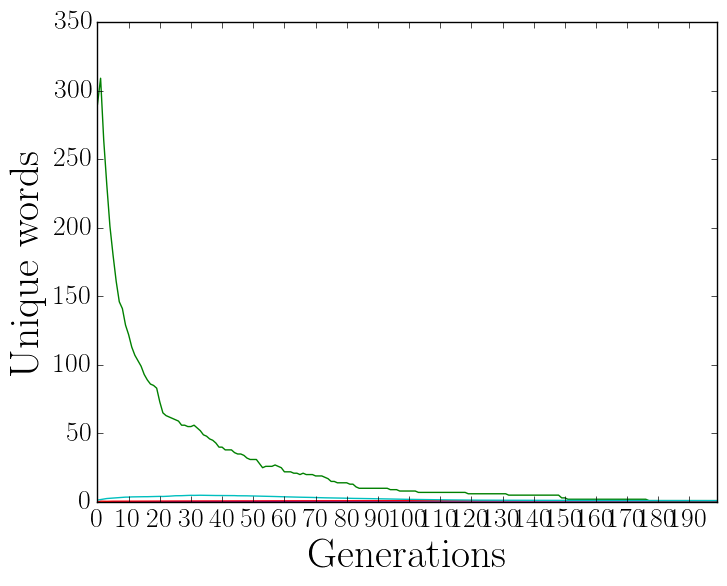
\includegraphics[width=0.49\linewidth]{fig/Results/Exp6.1/Vocabulary1}}
    \hfill
    \subfigure[Green: Average probability of conducting parent-child dialogues. Blue: Average learning rate. Red: Average probability of acting extrovertly.]{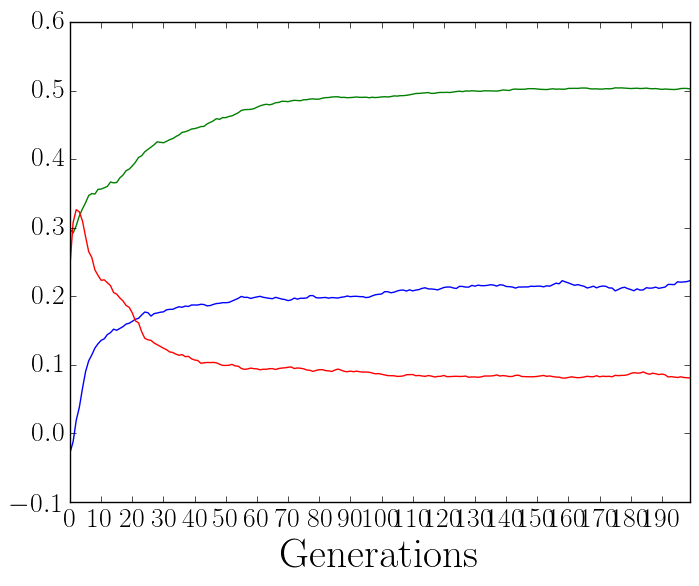
\includegraphics[width=0.49\linewidth]{fig/Results/Exp6.1/Genes1}}
    \caption{Graphs from experiment 6 with  $k = 0.95$ and $n = 0.85$.}
\end{figure}
\begin{figure}
    \subfigure[The social network at generation 5.]{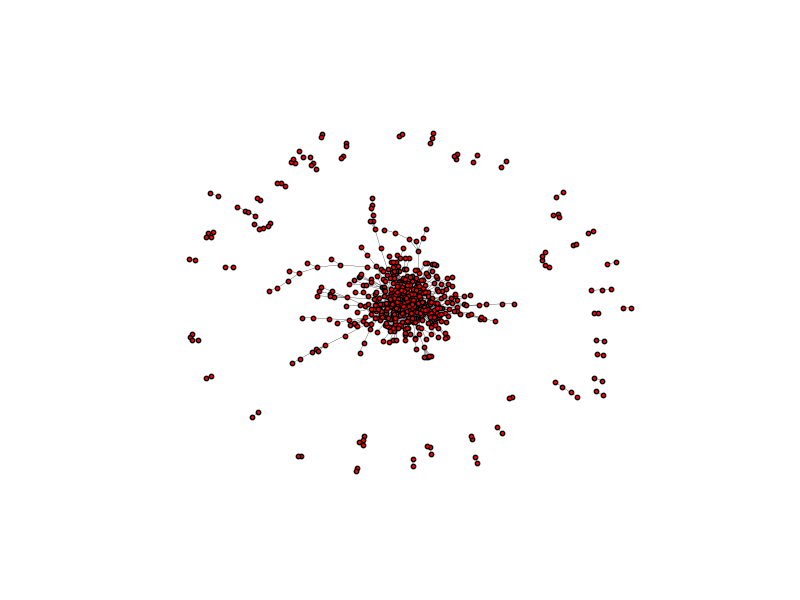
\includegraphics[width=0.49\linewidth]{fig/Results/Exp6.1/_graph5}}
    \hfill
    \subfigure[The social network at generation 20.]{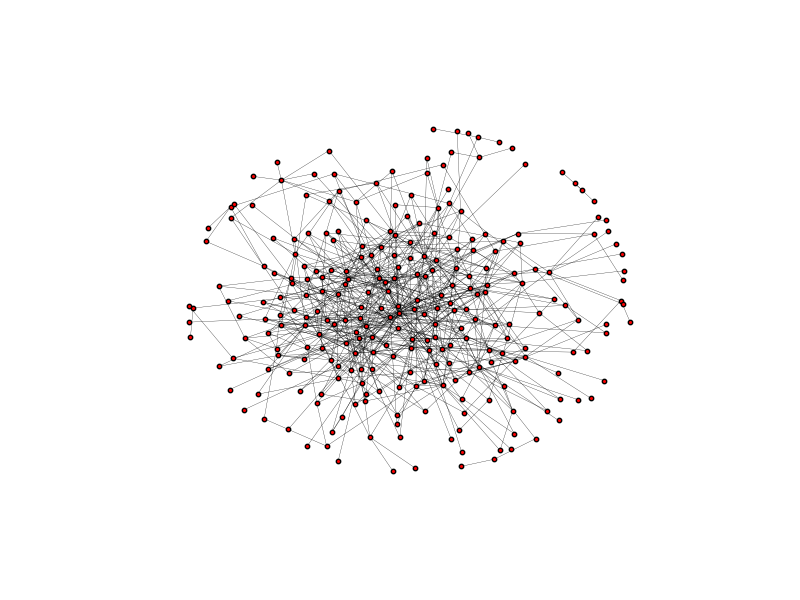
\includegraphics[width=0.49\linewidth]{fig/Results/Exp6.1/_graph20}}
    \par \bigskip
    \subfigure[The social network at generation 100.]{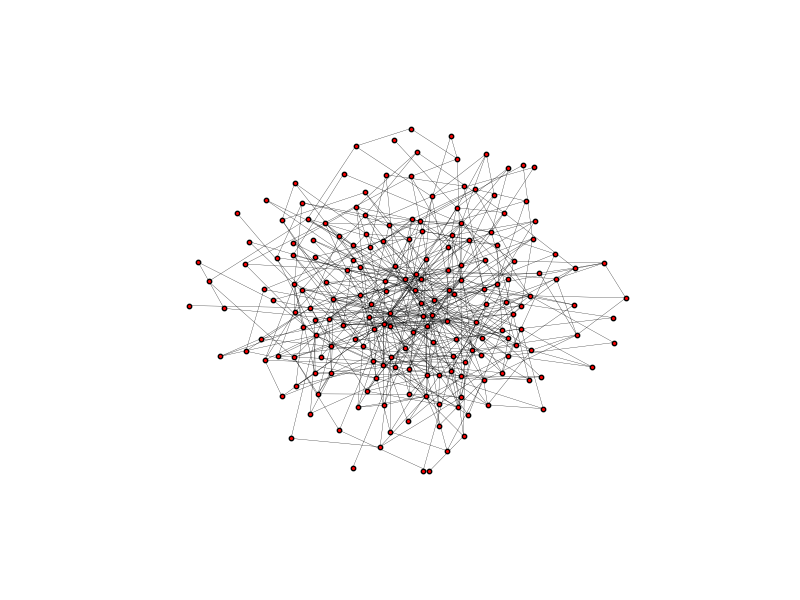
\includegraphics[width=0.49\linewidth]{fig/Results/Exp6.1/_graph100}}
    \caption{Social networks from experiment 6 with  $k = 0.95$ and $n = 0.85$.}
\end{figure}

\clearpage
\section{Experiment 7}
\begin{figure}[htbp]
    \centering
    \subfigure[Green: Average probability of conducting parent-child dialogues. Blue: Average learning rate. Red: Average probability of acting extrovertly.]{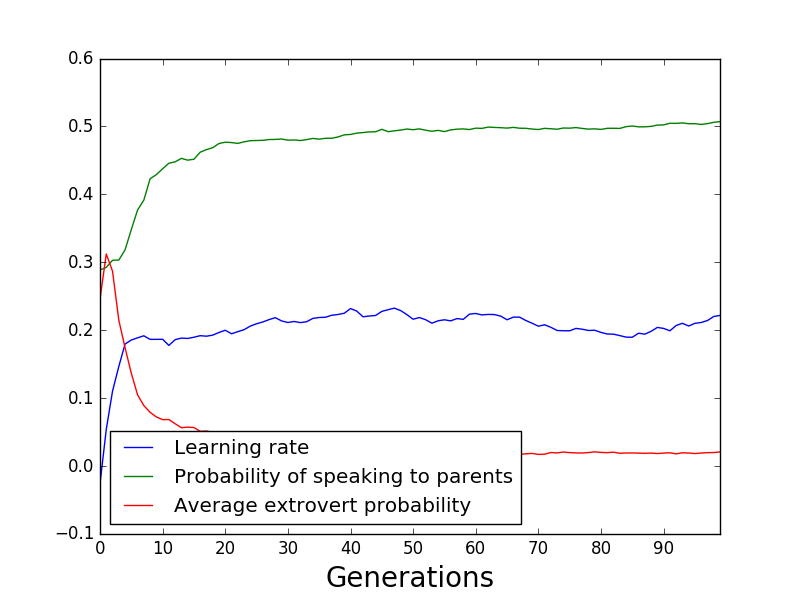
\includegraphics[width=0.5\linewidth]{fig/Results/Exp7/Genes1}}
    \hfill
    \subfigure[The social network at generation 5.]{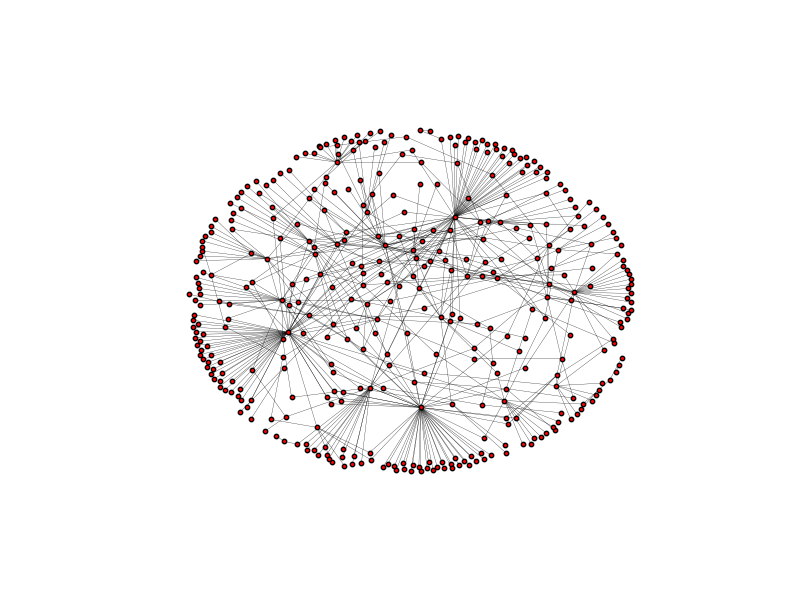
\includegraphics[width=0.49\linewidth]{fig/Results/Exp7/_graph5}}
    \par \bigskip
    \subfigure[The social network at generation 20.]{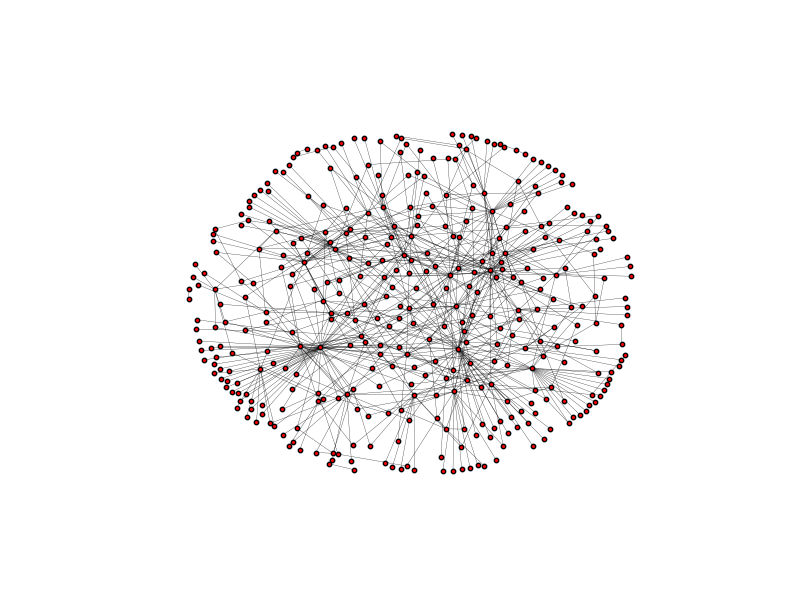
\includegraphics[width=0.49\linewidth]{fig/Results/Exp7/_graph20}}
    \hfill
    \subfigure[The social network at generation 100.]{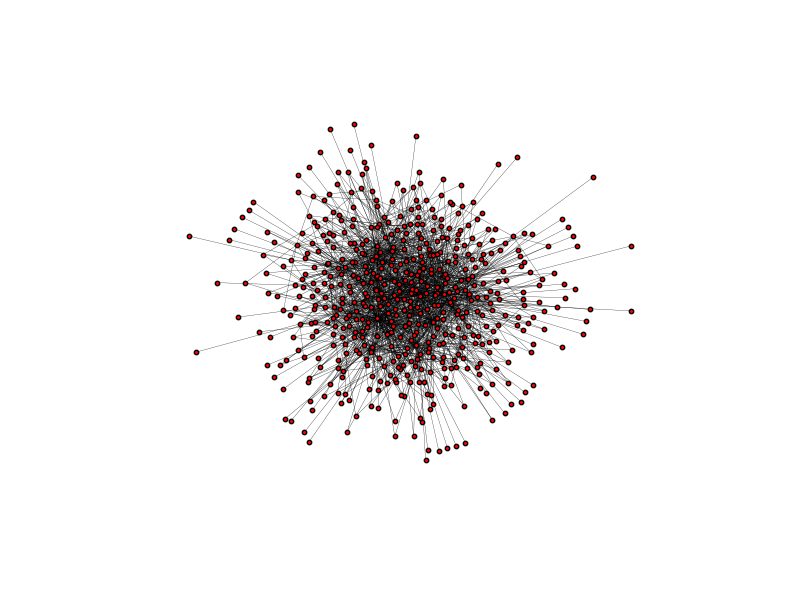
\includegraphics[width=0.49\linewidth]{fig/Results/Exp7/_graph100}}
    \caption{Results from experiment 7 with probability of inventing a word set to $25\%$.}
\end{figure}

\clearpage
\begin{figure}[htbp]
    \centering
    \subfigure[The average fitness.]{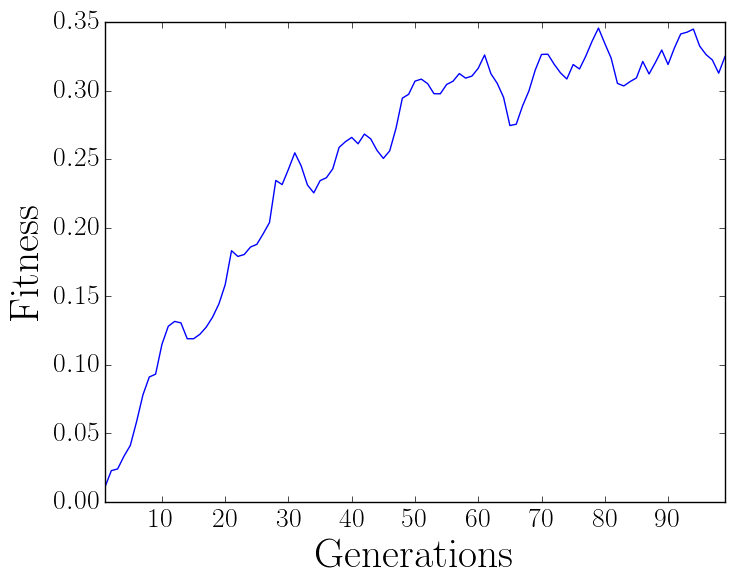
\includegraphics[width=0.49\linewidth]{fig/Results/Exp7.1/Fitness1}}
    \hfill
    \subfigure[The average degree.]{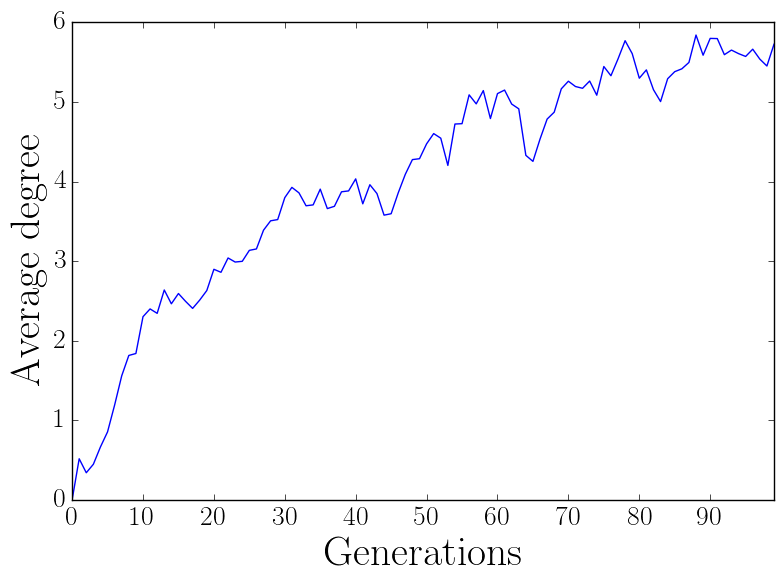
\includegraphics[width=0.49\linewidth]{fig/Results/Exp7.1/Degree1}}
    \par \bigskip
    \subfigure[Green: Average vocabulary size. Blue: Successful dialogues divided by total number of dialogues.]{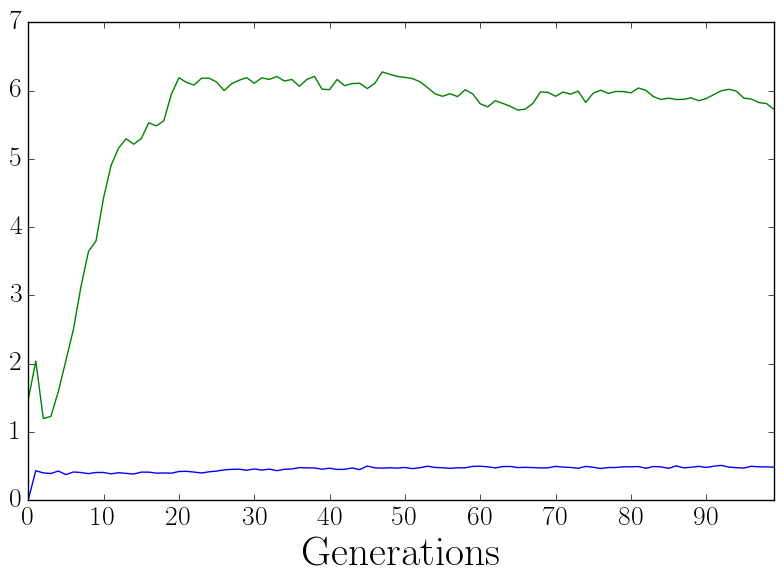
\includegraphics[width=0.49\linewidth]{fig/Results/Exp7.1/Vocabulary1}}
    \hfill
    \subfigure[Green: Average probability of conducting parent-child dialogues. Blue: Average learning rate. Red: Average probability of acting extrovertly.]{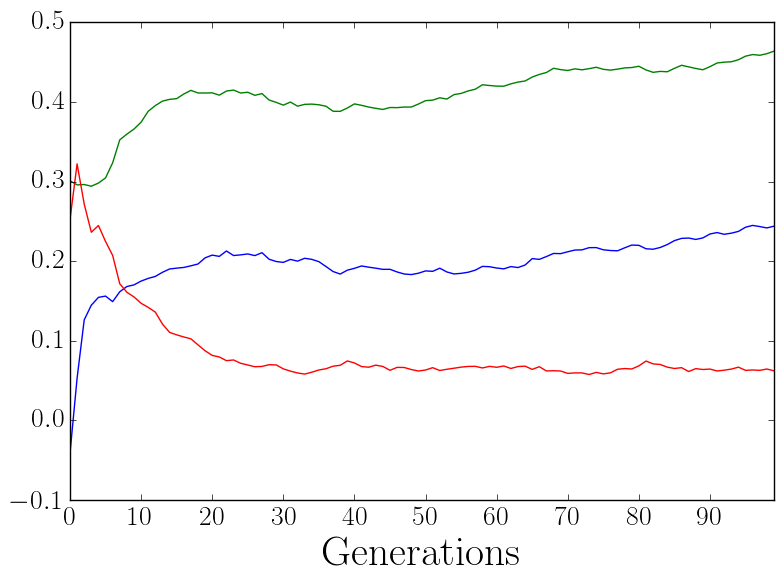
\includegraphics[width=0.49\linewidth]{fig/Results/Exp7.1/Genes1}}
    \caption{Results from experiment 7 with probability of inventing a word set to $45\%$.}
\end{figure}
\begin{figure}
    \subfigure[The social network at generation 5.]{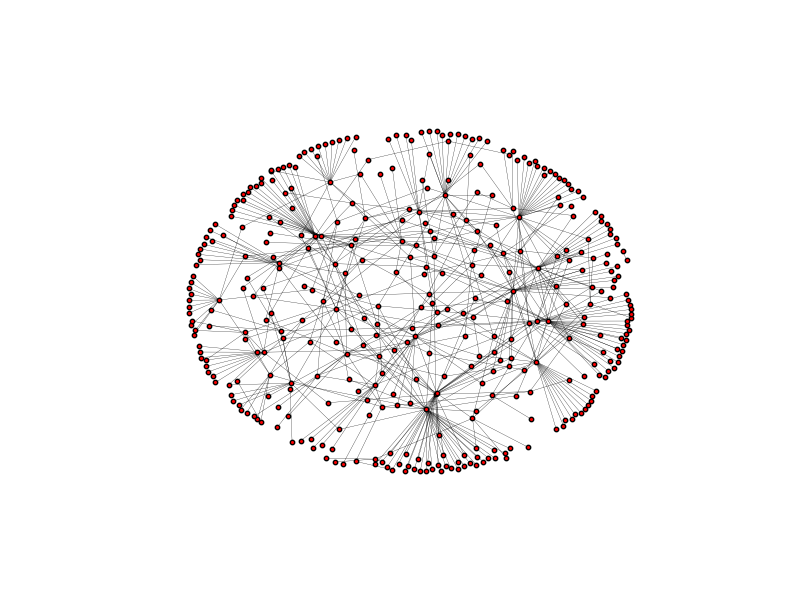
\includegraphics[width=0.49\linewidth]{fig/Results/Exp7.1/_graph5}}
    \hfill
    \subfigure[The social network at generation 20.]{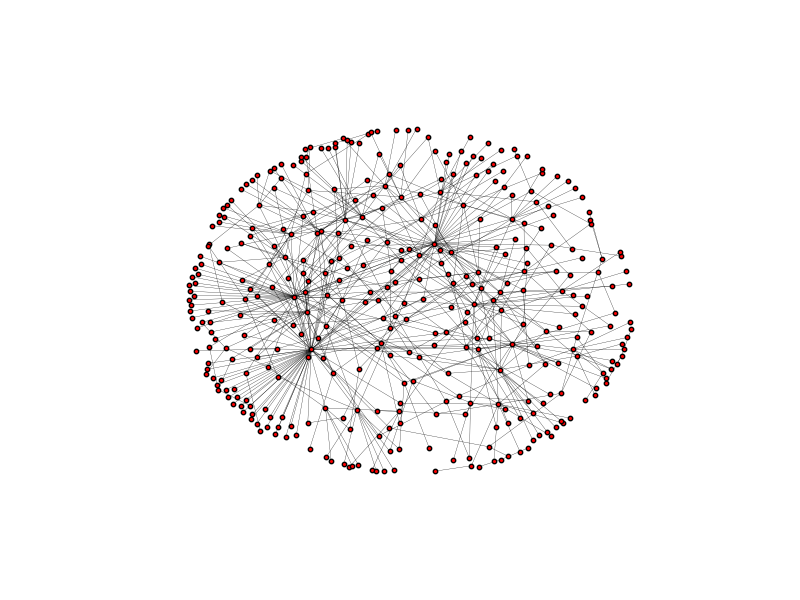
\includegraphics[width=0.49\linewidth]{fig/Results/Exp7.1/_graph20}}
    \par \bigskip
    \subfigure[The social network at generation 100.]{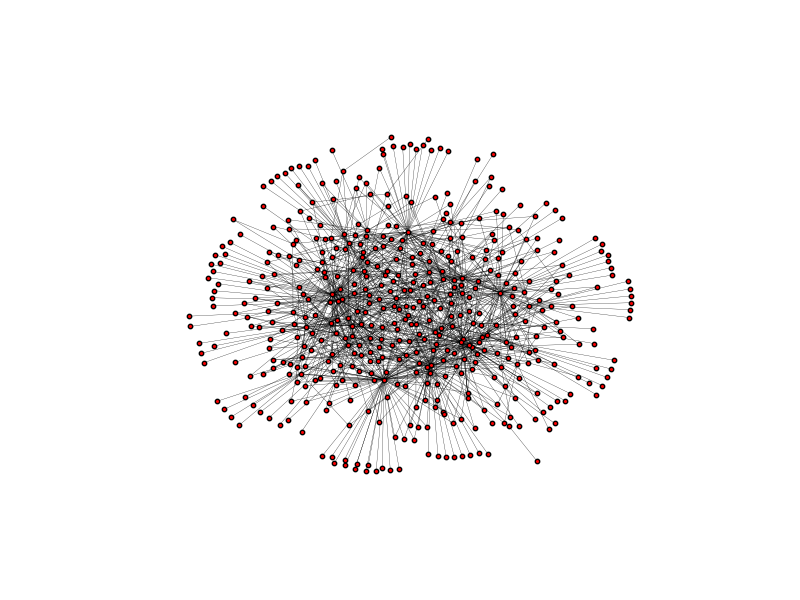
\includegraphics[width=0.49\linewidth]{fig/Results/Exp7.1/_graph100}}
    \caption{Results from experiment 7 with probability of inventing a word set to $45\%$.}
\end{figure}